\documentclass[tikz, border=5pt]{standalone}
\usetikzlibrary{shapes,arrows,positioning}

\begin{document}
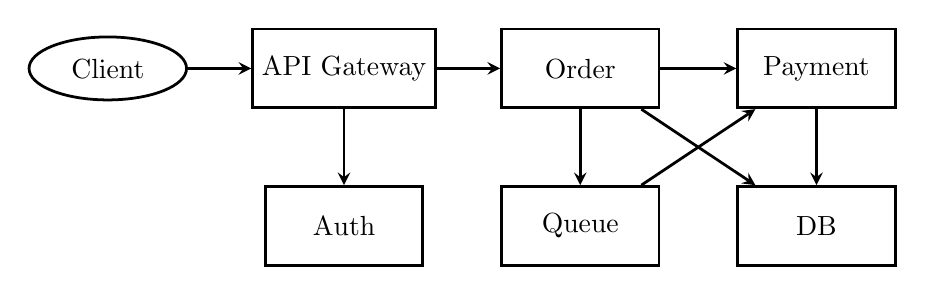
\begin{tikzpicture}[
  block/.style={rectangle, draw, minimum width=2cm, minimum height=1cm},
  oval/.style={ellipse, draw, minimum width=2cm, minimum height=0.8cm},
  ->, >=stealth, line width=1pt
]

\node[oval] (client) at (0, 2) {Client};
\node[block] (gateway) at (3, 2) {API Gateway};
\node[block] (auth) at (3, 0) {Auth};
\node[block] (order) at (6, 2) {Order};
\node[block] (payment) at (9, 2) {Payment};
\node[block] (queue) at (6, 0) {Queue};
\node[block] (db) at (9, 0) {DB};

\draw (client) -- (gateway);
\draw (gateway) -- (auth);
\draw (gateway) -- (order);
\draw (order) -- (payment);
\draw (order) -- (queue);
\draw (queue) -- (payment);
\draw (payment) -- (db);
\draw (order) -- (db);

\end{tikzpicture}
\end{document}
